\section {Detaching neighboring meshes}
Alternatively, instead of merging neighboring intersecting meshes, we can also remove intersections by cutting the mesh into individual components. This approach is required for specific applications. For example, when using FEM to solve an equation that describes a physics problem, each component needs to be assigned its own physical properties (e.g., electric conductivity) and thus its boundaries need to be clearly defined. A different example is the brain model described before, in which the individual gyri of one mesh may intersect. While they are not physically separate organs, each gyrus is an anatomical entity with its own function. Hence, an individual, intersection-free mesh representation of each gyrus might be needed, for example, in high resolution FEM. In addition, the local directions of neurons are defined as perpendicular to the surface, so directions remain unknown in areas without a surface. We did not find any methods that solve this problem. Here we present our implementation. It first cuts an intersecting mesh into submeshes by removing self-intersecting facets. That removal may introduce holes and small floating components. Next, the method retains only the primary submeshes of interest, and discards the rest. The resulting holes are then patched. While this method does not preserve the original geometry, its main goal is to differentiate submeshes that are meant to represent different entities. Figure \ref{fig:sol3-2} shows the original and repaired mesh for Test Case 1. Our method produced
geometrically correct meshes of reasonable quality. Another test case is presented in the supplemental material. We aim to further improve this method to produce higher quality results.

\vspace{-0.5em}

\begin{figure}[h]
    \centering
    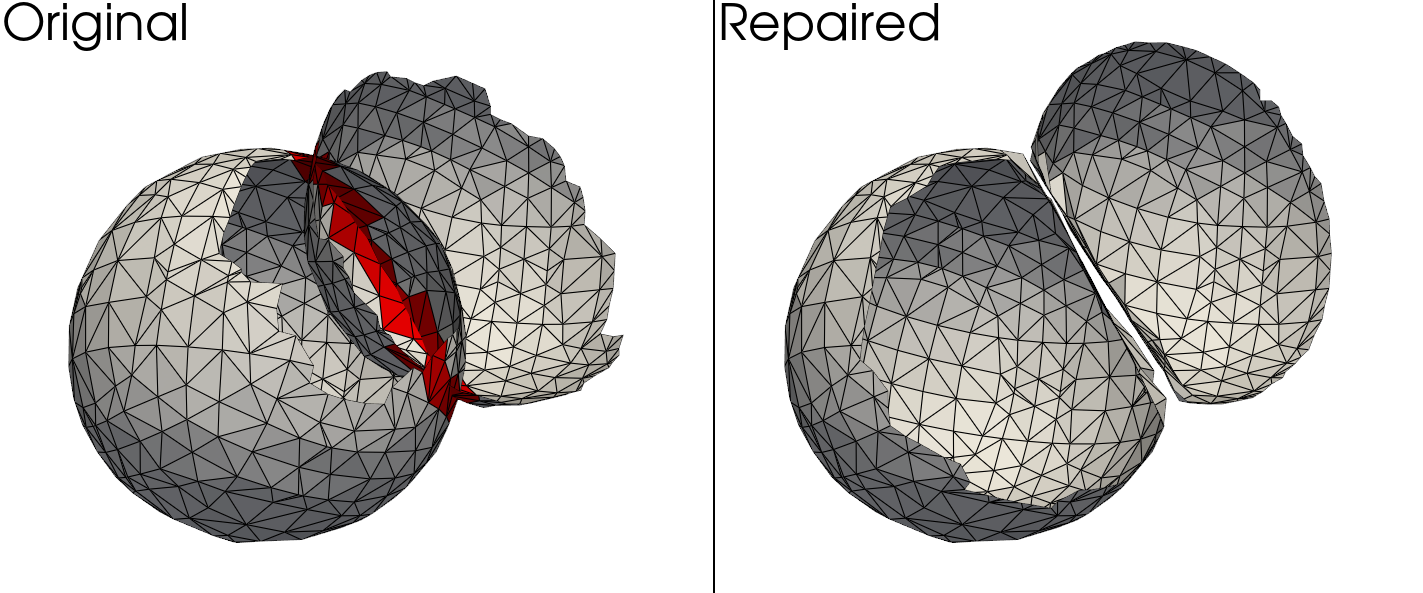
\includegraphics[width=0.6\linewidth, height=2.2cm]{../figures/detach_n_1.png}
    \caption{\textbf{Detaching neighboring meshes.} Original and repaired mesh for test case 1. The meshes have been divided into two distinct pieces, as opposed to the solution shown in Fig. \ref{fig:sol2-2}.}
    \label{fig:sol3-2}
\end{figure}

\vspace{-1em}